\documentclass{article}

\usepackage[T1]{fontenc}
\usepackage{graphicx} % Required for inserting images
\usepackage[utf8]{inputenc}
\usepackage[polish]{babel}

\title{Lab4 - Sytem kontroli wersji git}
\author{Jakub Włodarczyk}
\date{04.11.2023}

\begin{document}

\maketitle

\section{Konfiguracja gita}

Jako że korzystam z systemu kontroli wersji git na codzień, nie chciałem przerpowadzać instalacji na nowo aby pokazywać na nowo jej etapy. Zmieniłem za to użytkownika poświadczeń na pocztę mailu uczelnianego aby spełnić wymagania określone w treści zadania. 

\begin{figure}[!h]
    \caption{Konfiguracja GIT}
    \centerline{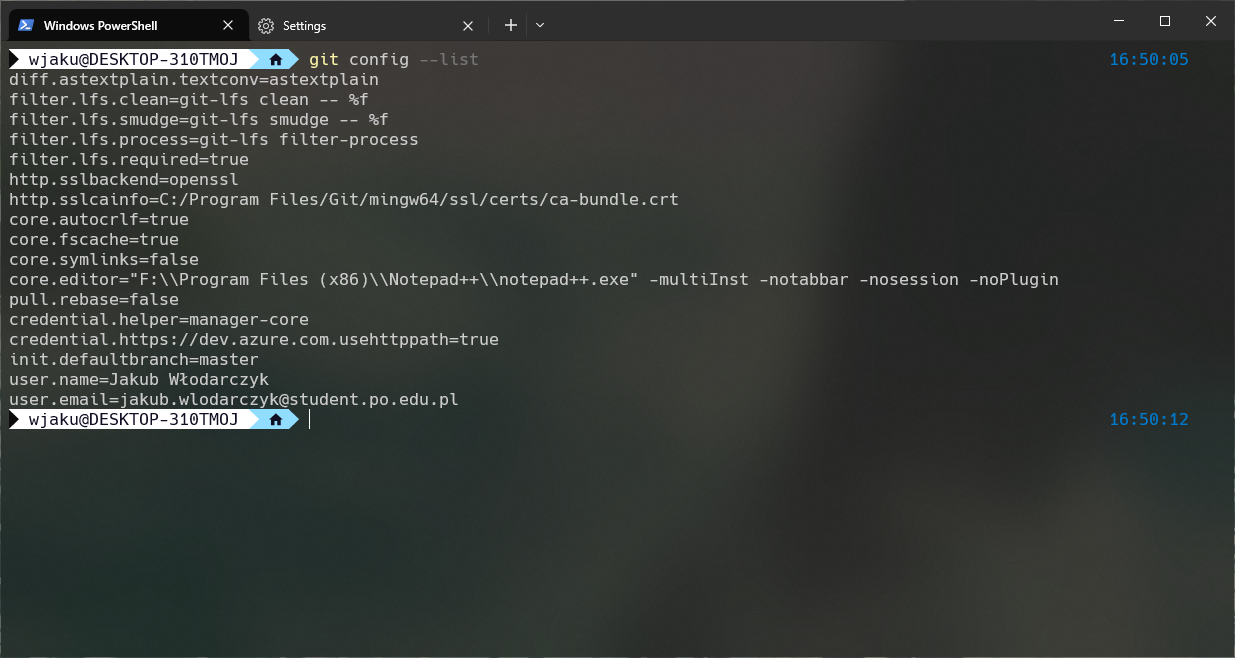
\includegraphics [scale=0.5]{config.PNG}}
    \label{fig:label}
\end{figure}
\newpage

\section{Inicjalizacja repozytorium}

Utworzenie katalogu na poczet wykonania laboratorium, oraz inicjalizacja repozytorium.

\vspace*{\fill}
\begin{figure}[!h]
    \caption{Inicjalizacja repozytorium}
    \centerline{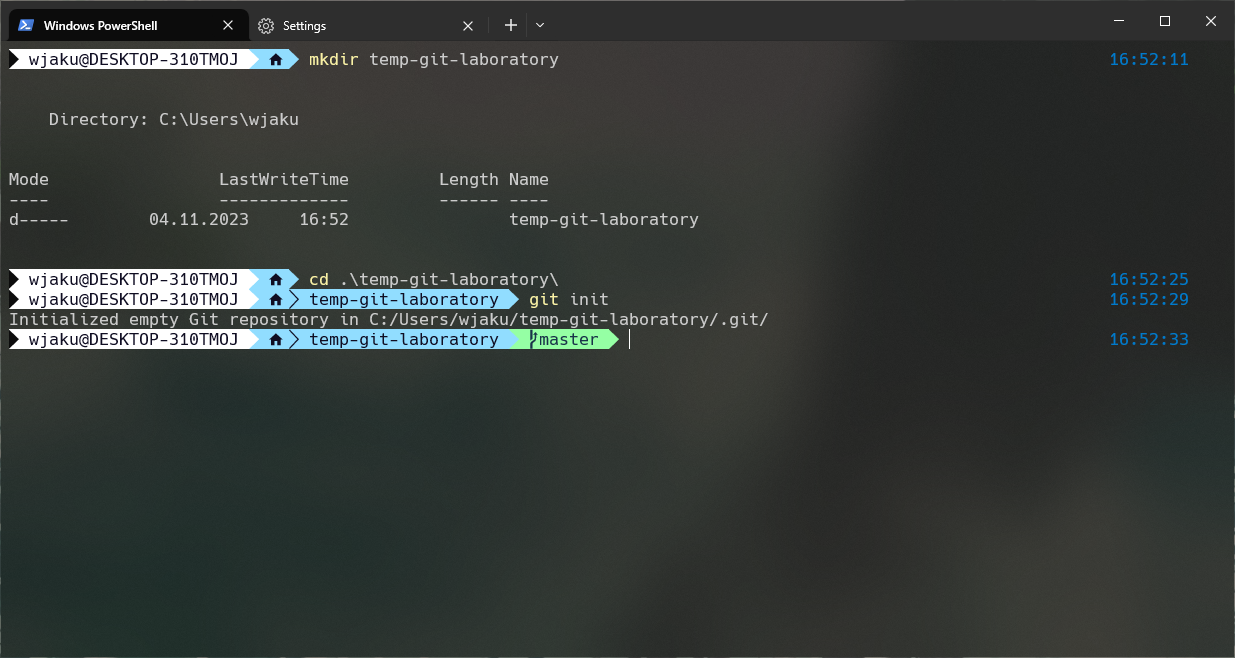
\includegraphics [scale=0.5]{git-init.PNG}}
    \label{fig:label}
\end{figure}
\vspace*{\fill}
\newpage

\section{Dodanie podstawowych plików}

Utworzenie plików, w swoim przykładzie będę korzystał z plików .cs które są rozszerzeniem stosowanym do określenie plików z kodem Csharp.

\vspace*{\fill}
\begin{figure}[!h]
    \caption{Dodanie podstawowych plików}
    \centerline{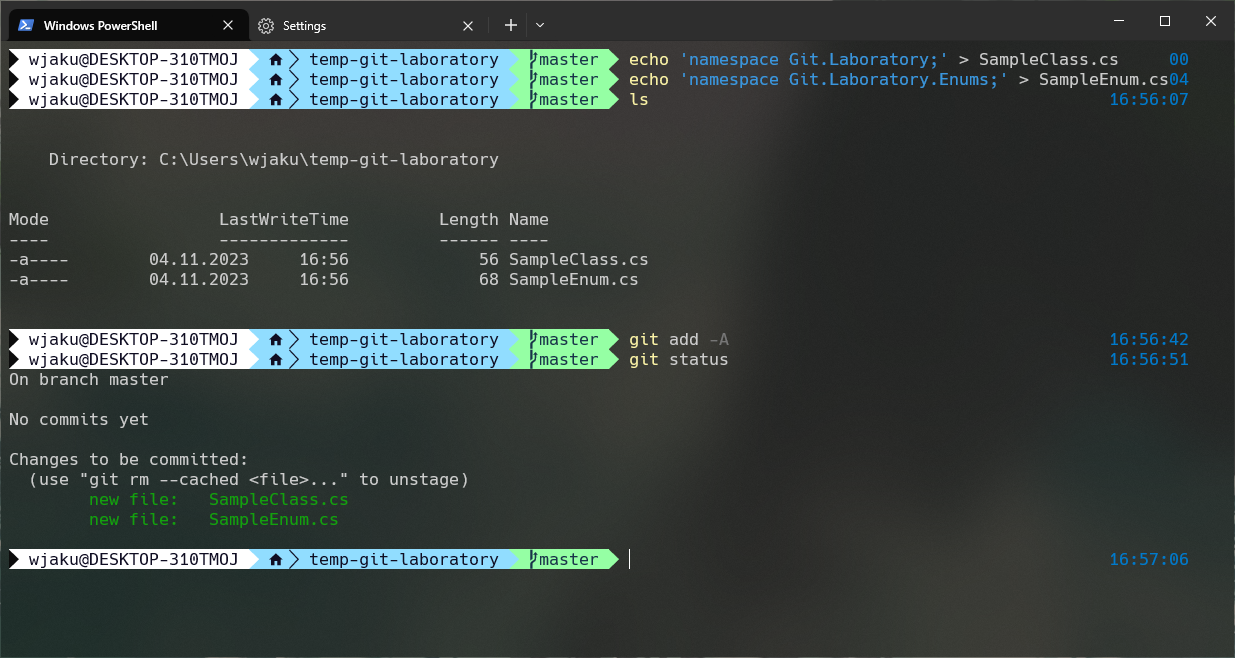
\includegraphics [scale=0.5]{files-initialization.PNG}}
    \label{fig:label}
\end{figure}
\vspace*{\fill}
\newpage

\section{Modyfikacje plików w przestrzeni Stage}

Segment przedstawia parę zmian dokonanych na plikach, oraz wyniki tych zmian w systemie kontroli wersji.

\vspace*{\fill}
\begin{figure}[!h]
    \caption{Zmiana pliku SampleClass.cs }
    \centerline{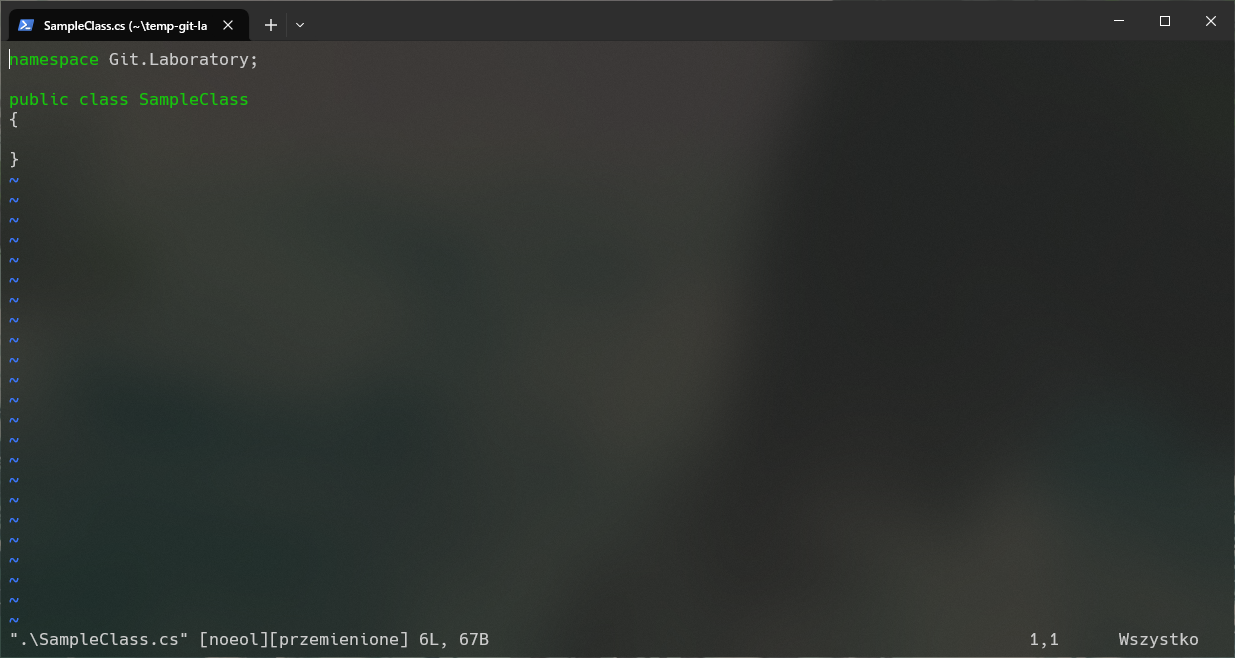
\includegraphics [scale=0.5]{smapleClass-CHange.PNG}}
    \label{fig:label}
\end{figure}
\vspace*{\fill}
\newpage

\vspace*{\fill}
\begin{figure}[!h]
    \caption{Rezultat zmiany pliku SampleClass.cs }
    \centerline{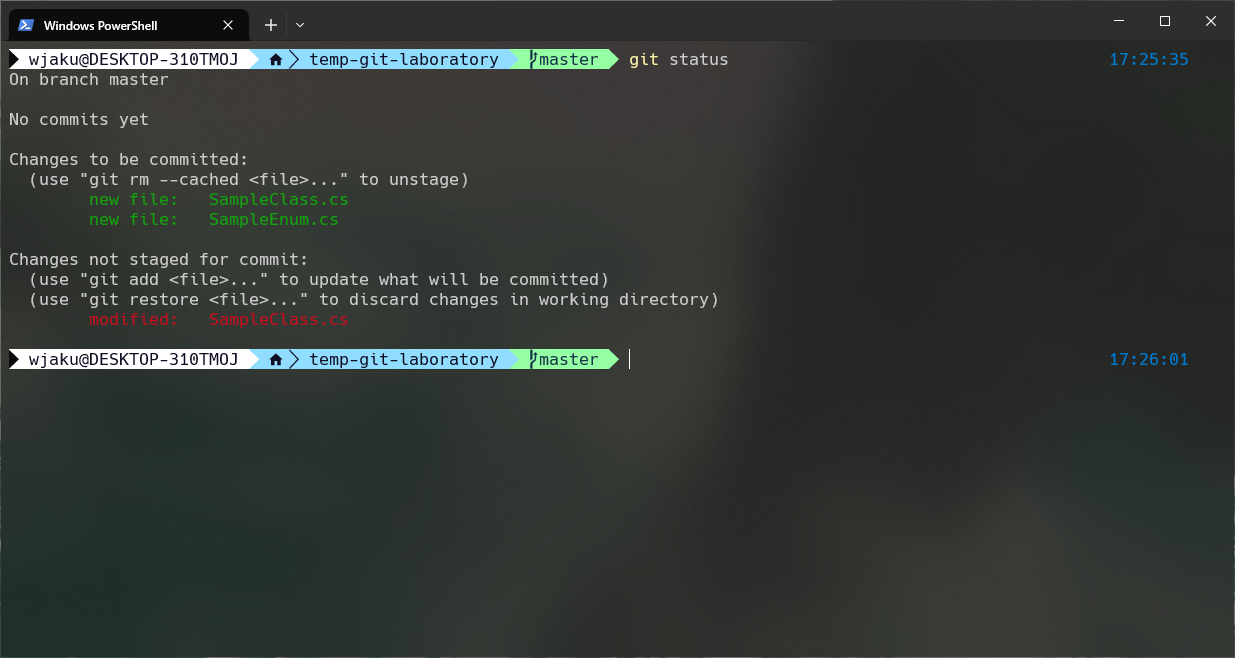
\includegraphics [scale=0.5]{sampleClass-modifited.PNG}}
    \label{fig:label}
\end{figure}
\vspace*{\fill}

\newpage

\vspace*{\fill}
\begin{figure}[!h]
    \caption{Zmiana nazwy pliku SampleEnum.cs }
    \centerline{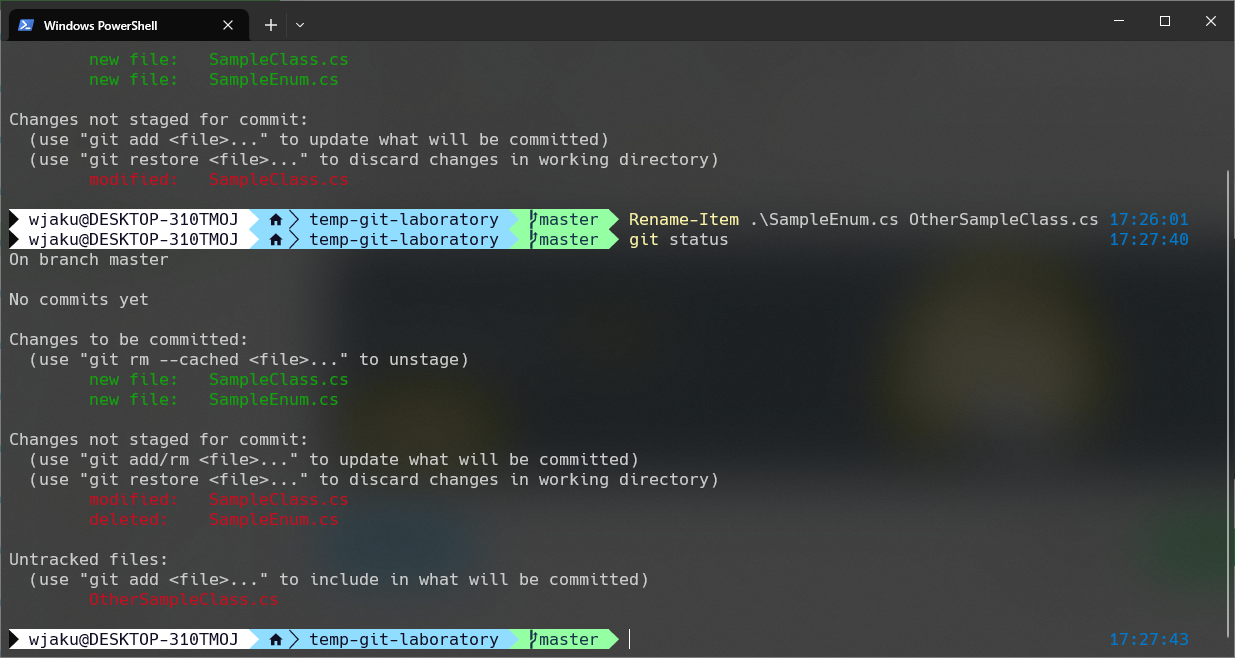
\includegraphics [scale=0.5]{rename-enum.PNG}}
    \label{fig:label}
\end{figure}
\vspace*{\fill}

\newpage

\vspace*{\fill}
\begin{figure}[!h]
    \caption{Usunięcie pliku OtherSampleEnum.cs }
    \centerline{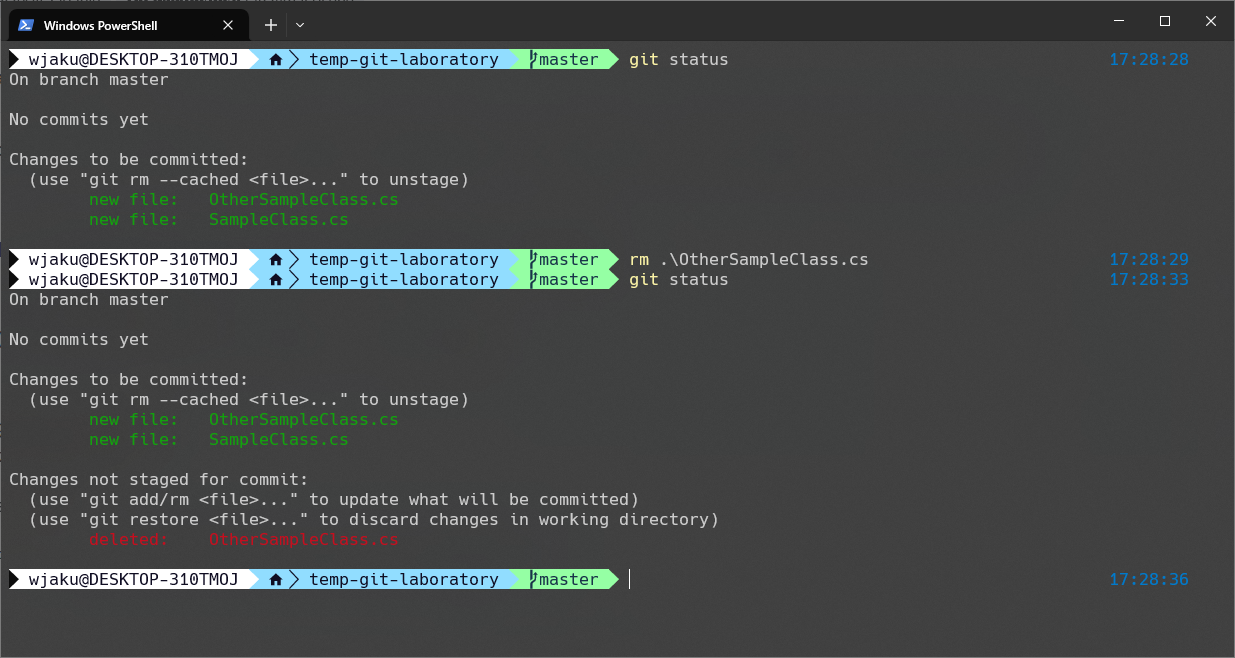
\includegraphics [scale=0.5]{remove-otherSampleClass.PNG}}
    \label{fig:label}
\end{figure}
\vspace*{\fill}
\newpage

\section{Utworzenie rewizji}

Zgodnie z treścią zadania dodane zostaną rewizje w celu lepszego ukazania dalszych kroków zadania.

\vspace*{\fill}
\begin{figure}[!h]
    \caption{Utworzenie pierwszego commita}
    \centerline{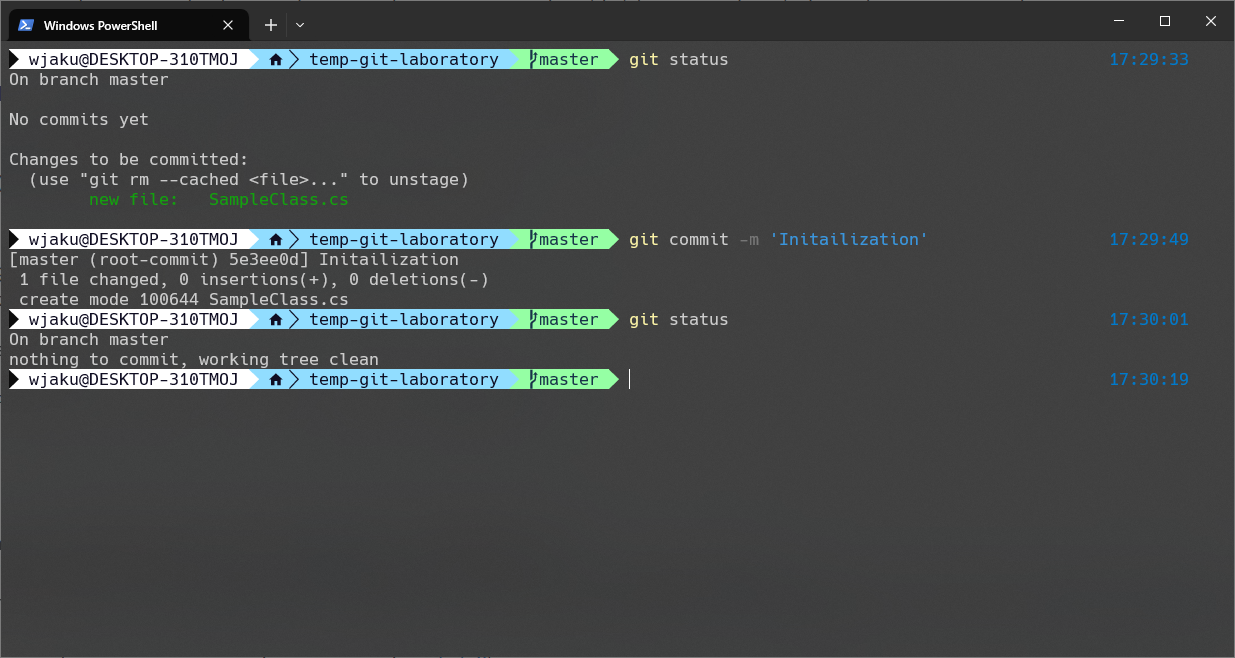
\includegraphics [scale=0.5]{initialization-commit.PNG}}
    \label{fig:label}
\end{figure}
\vspace*{\fill}
\newpage

\vspace*{\fill}
\begin{figure}[!h]
    \caption{Utworzenie interfejsu połączenia do bazy danych}
    \centerline{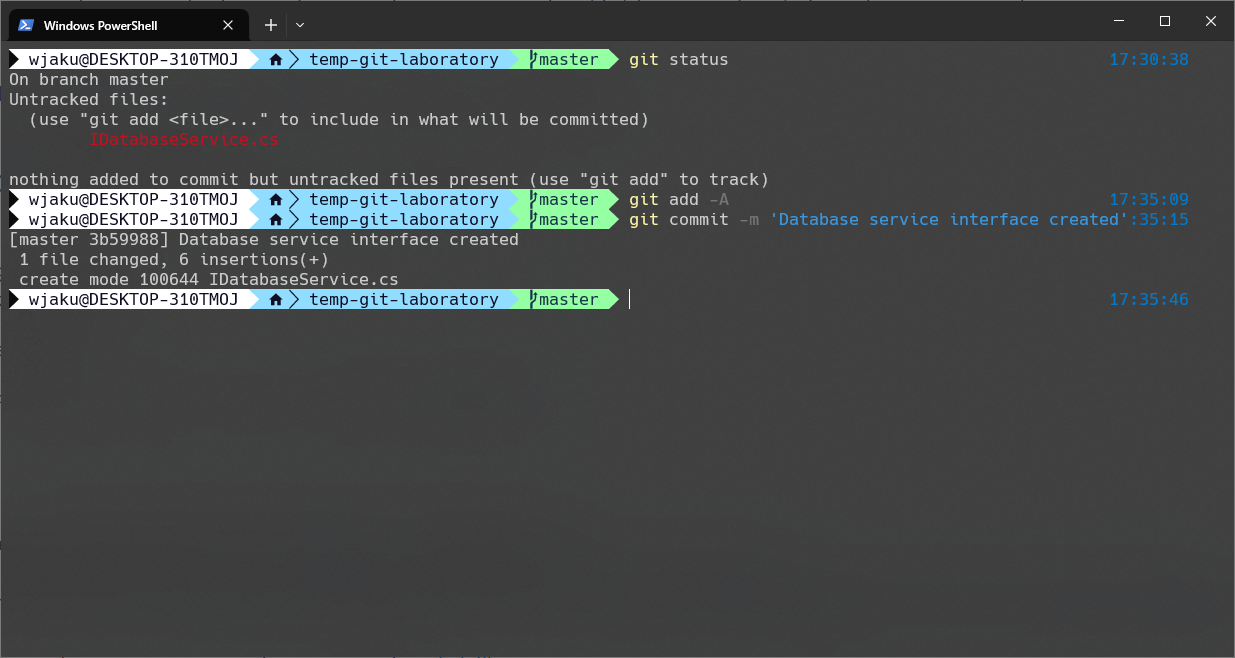
\includegraphics [scale=0.5]{database-service-interface.PNG}}
    \label{fig:label}
\end{figure}
\vspace*{\fill}
\newpage

\vspace*{\fill}
\begin{figure}[!h]
    \caption{Implementacja interfejsu połączenia do bazy danych}
    \centerline{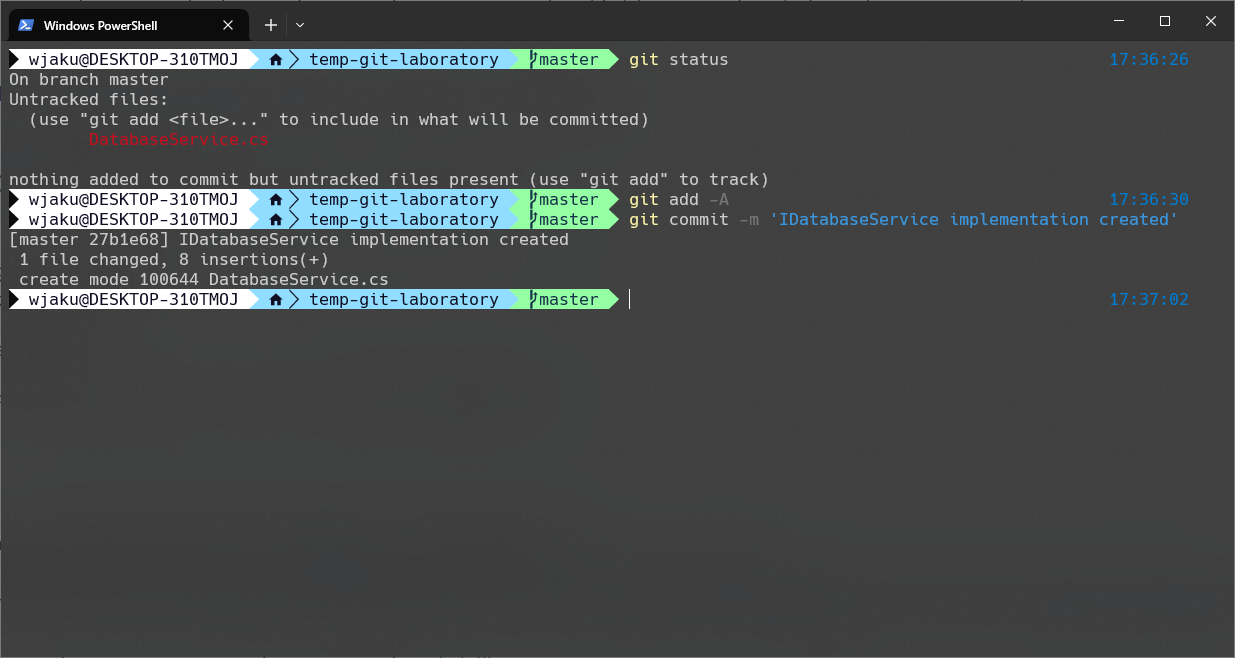
\includegraphics [scale=0.5]{database-service-implementation.PNG}}
    \label{fig:label}
\end{figure}
\vspace*{\fill}
\newpage

\vspace*{\fill}
\begin{figure}[!h]
    \caption{Wynik utworzenia powyższych rewizji}
    \centerline{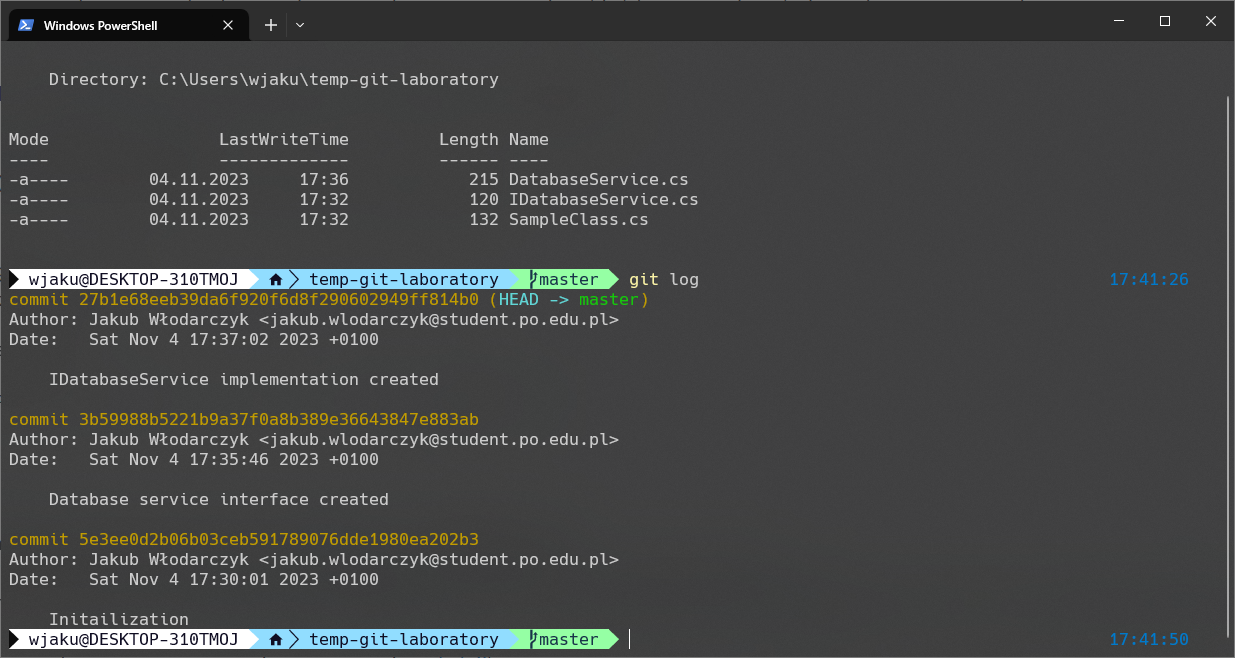
\includegraphics [scale=0.5]{first-log.PNG}}
    \label{fig:label}
\end{figure}
\vspace*{\fill}
\newpage

\section{Ignorowanie plików oraz katalogów z wykorzystaniem .gitignore}

Utworzenie pliku .gitignore w celu wykluczenia konkretnych katalogów z przestrzeni śledzonych plików repozytorium.

\vspace*{\fill}
\begin{figure}[!h]
    \caption{Utworzenie pliku .gitignore}
    \centerline{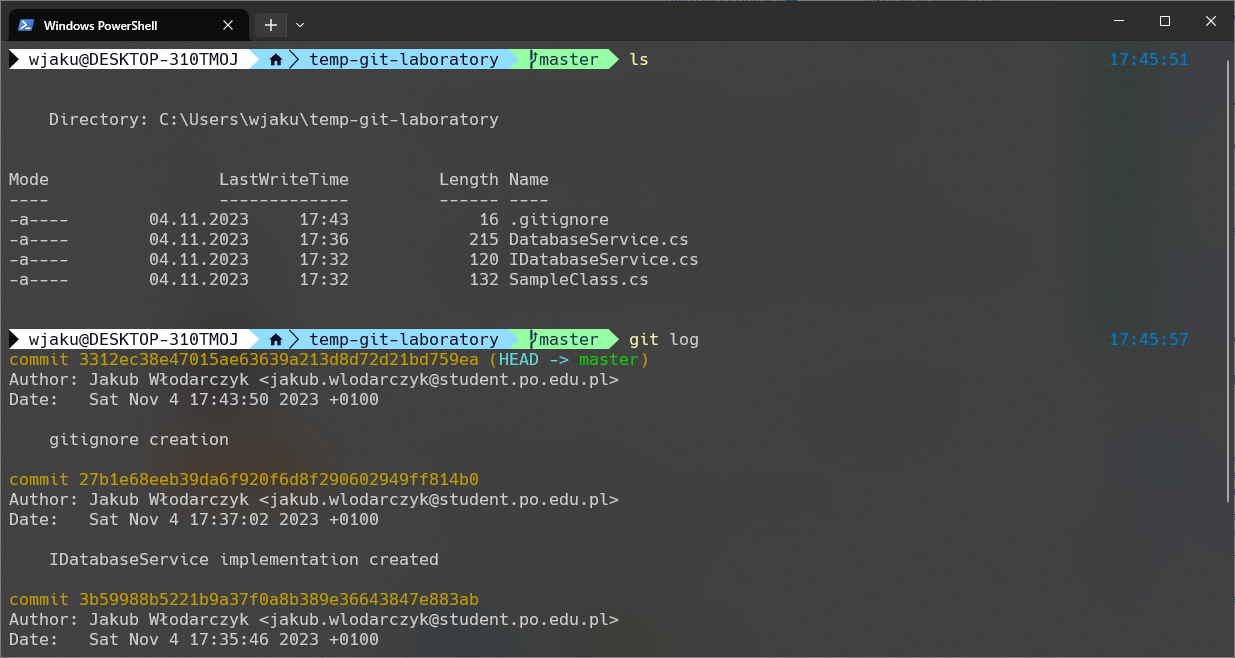
\includegraphics [scale=0.5]{gitignore-creation.PNG}}
    \label{fig:label}
\end{figure}
\vspace*{\fill}
\newpage

\vspace*{\fill}
\begin{figure}[!h]
    \caption{Zawartość pliku .gitignore}
    \centerline{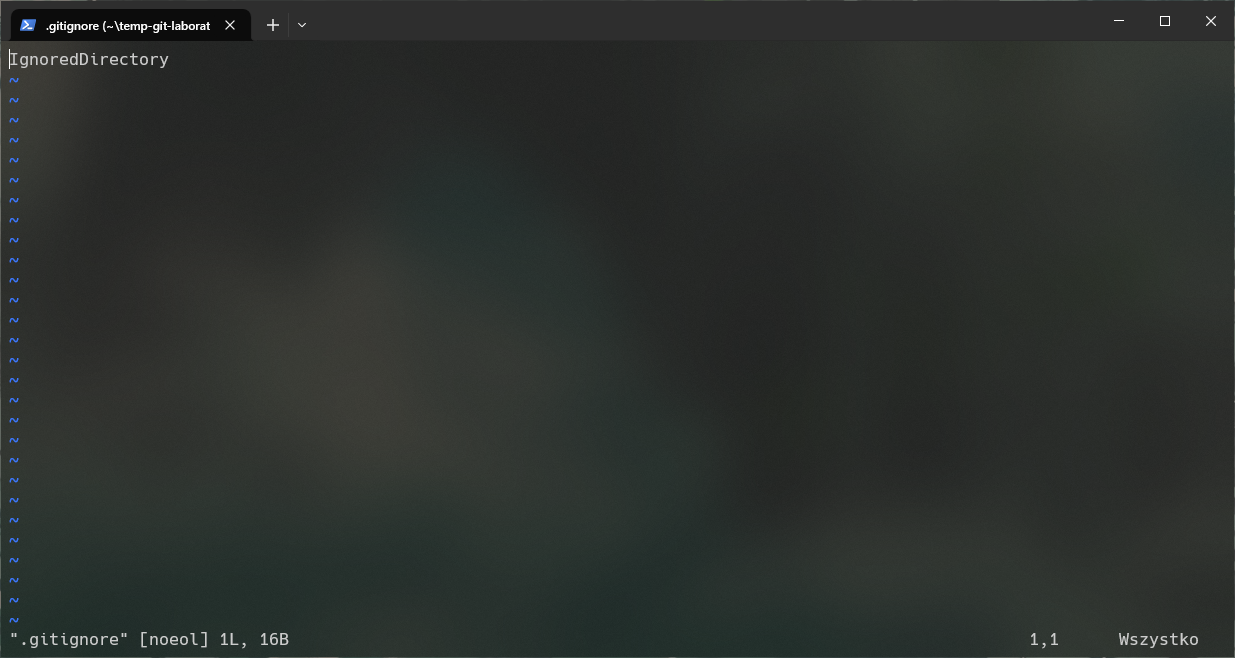
\includegraphics [scale=0.5]{gitignore.PNG}}
    \label{fig:label}
\end{figure}
\vspace*{\fill}
\newpage

\vspace*{\fill}
\begin{figure}[!h]
    \caption{Ignorowanie katalogu przy użyciu pliku .gitignore}
    \centerline{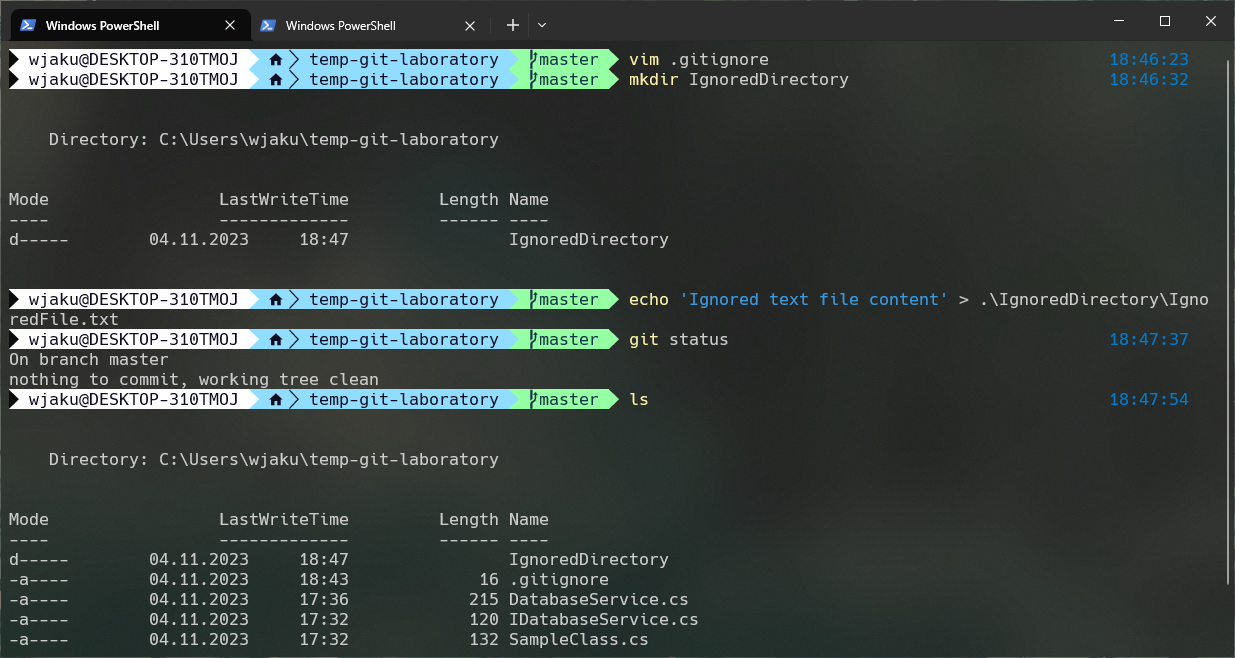
\includegraphics [scale=0.5]{gitignore-working.PNG}}
    \label{fig:label}
\end{figure}
\vspace*{\fill}
\newpage

\section{Poprawki w strukturze rewizji}

Podczas wykonywania ćwiczenia natrafiłem na błąd w którym plik .gitignore niepoprawnie reagował na swoją zawartość nie wykluczając wskazanego katalogu. W procesie weryfikacji przyczyny tego błędu zostało utworzone pare commitów które nie przyniosły żadnego poprawnego rezultatu i byłyby zbędne w całym ciagu rewizji repozytorium, dlatego dokonałem ich wyczyszczenia. 

\vspace*{\fill}
\begin{figure}[!h]
    \caption{Reflog rewizji przed dokonaniem wyczyszenia}
    \centerline{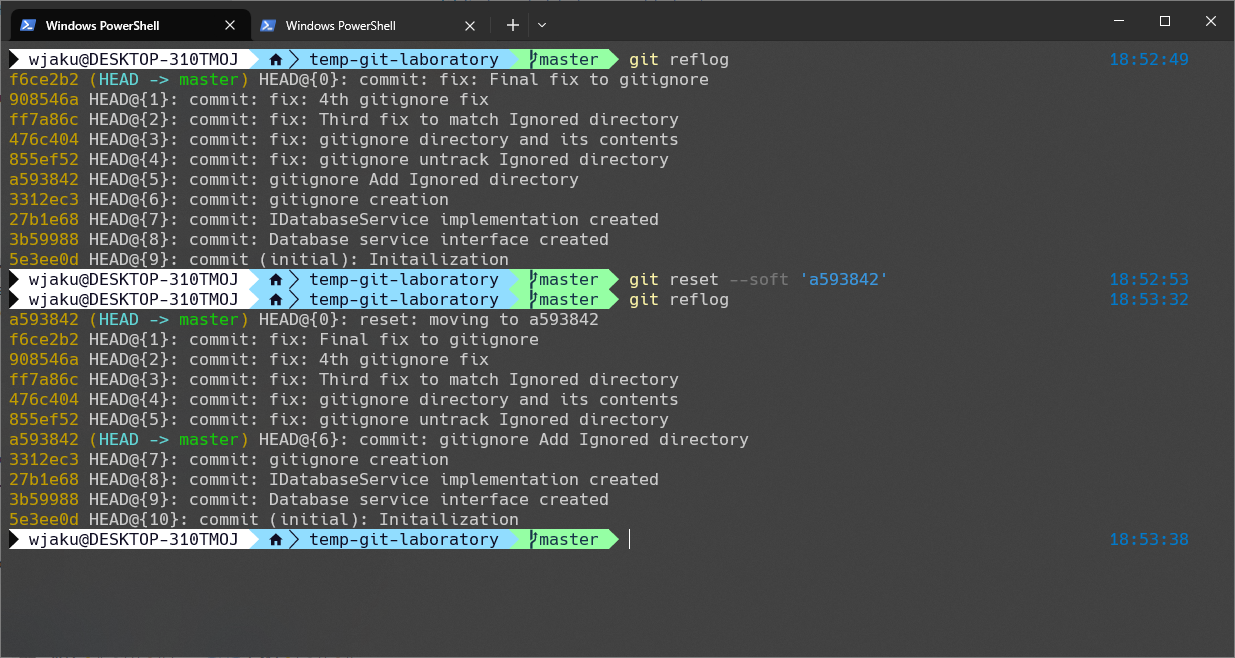
\includegraphics [scale=0.5]{before-squash.PNG}}
    \label{fig:label}
\end{figure}
\vspace*{\fill}
\newpage

\vspace*{\fill}
\begin{figure}[!h]
    \caption{Spłaszczenie struktury rewizji repozytorium}
    \centerline{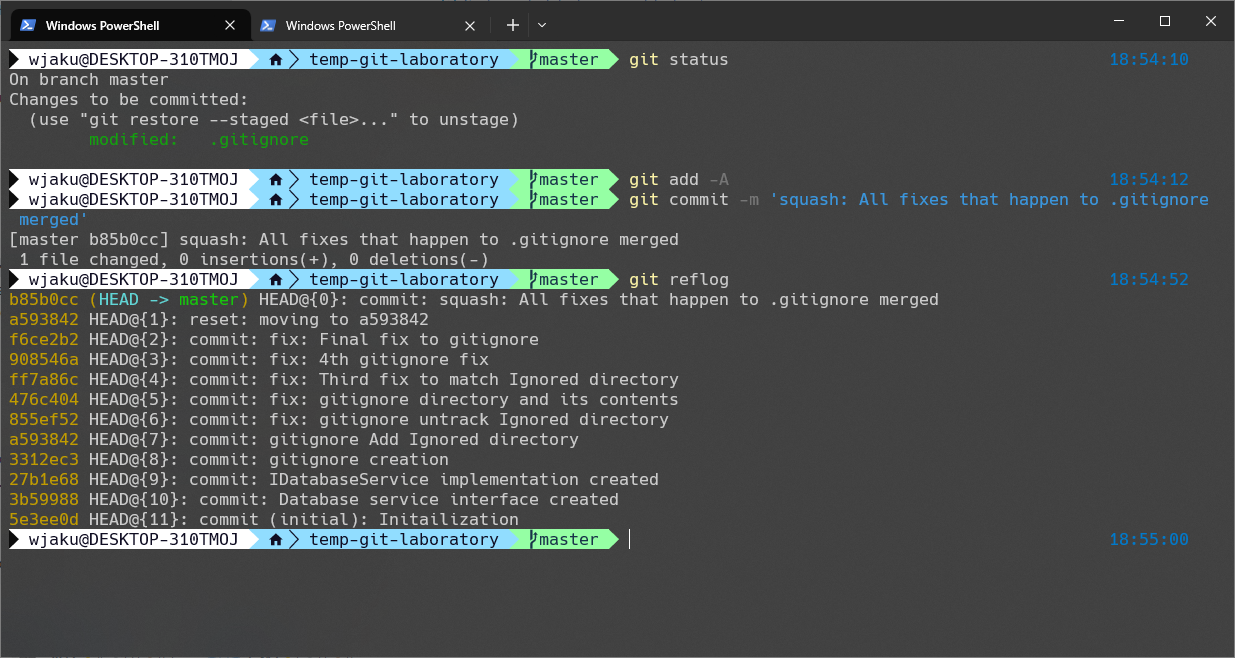
\includegraphics [scale=0.5]{squash.PNG}}
    \label{fig:label}
\end{figure}
Komenda reflog zwraca informacje na temat wszystkich rewizji dokananych w obrębie danej gałęzi, dlatego spłaszczenie będzie lepiej widoczne w kolejnym segmencie.
\vspace*{\fill}
\newpage

\section{Spis rewizji}

Do wyświetlania commitów repozytorium wykorzystuje alias który wyświetliłem na pierwszym zrzucie w znaczny sposób ułatwia on pracę z commitami, oraz czytelność ich struktury. 

\vspace*{\fill}
\begin{figure}[!h]
    \caption{Spis struktury commitów}
    \centerline{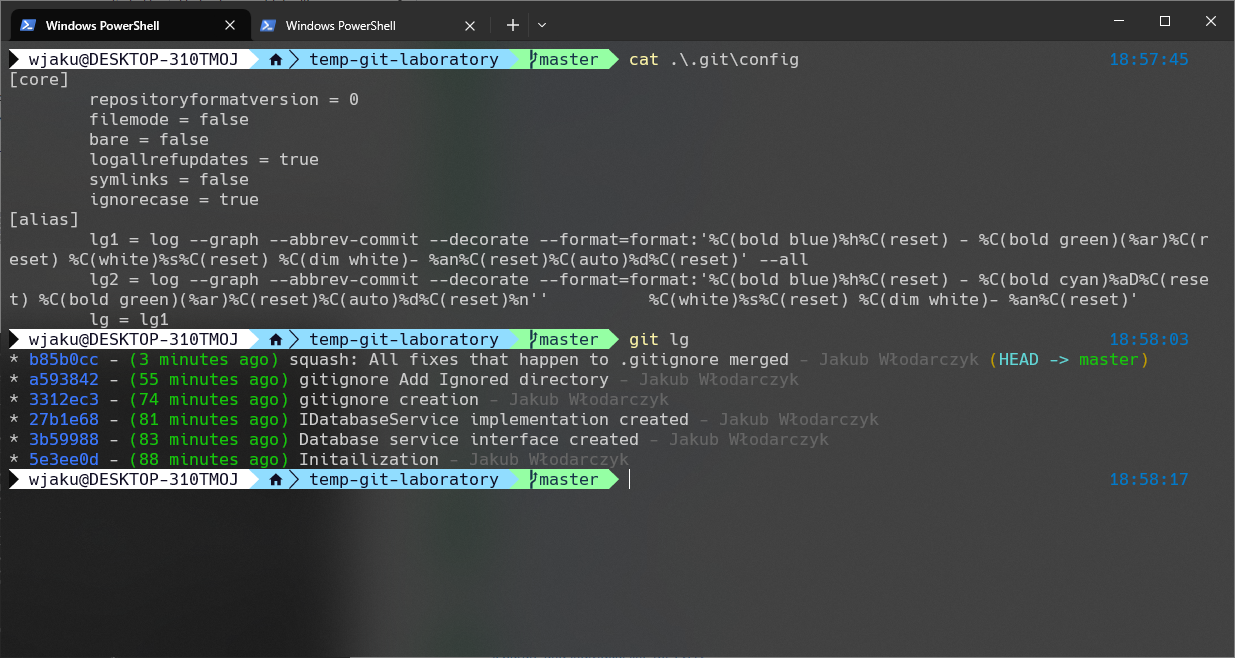
\includegraphics [scale=0.5]{readlible-log.PNG}}
    \label{fig:label}
\end{figure}
\vspace*{\fill}
\newpage

\section{Praca z gałeziami}

W ramach realizacji ćwiczenia został utworzony branch develop.

\vspace*{\fill}
\begin{figure}[!h]
    \caption{Utworzenie brancha develop}
    \centerline{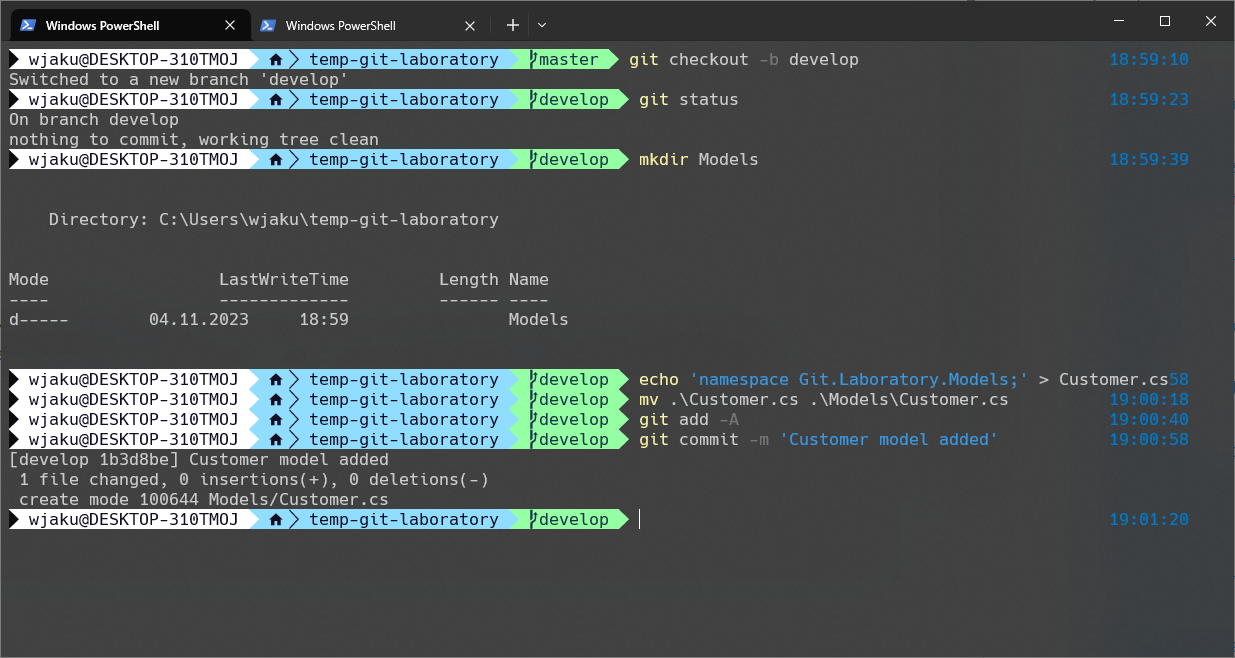
\includegraphics [scale=0.5]{customer-model.PNG}}
    \label{fig:label}
\end{figure}
\vspace*{\fill}
\newpage

\section{Róznica w plikach - git diff}

W celu ukazania działania komendy plik Customer.cs został zmieniony, niestety system kontroli wersji nie wspiera wyświetlania zmiany zawartości w plikach o rozszrzeniu .cs, jest to funkcjonalność dla plików tekstowych. (Pliki .cs są uznawane za binarne)

\vspace*{\fill}
\begin{figure}[!h]
    \caption{Zawartość pliku Customer.cs przed zmianą}
    \centerline{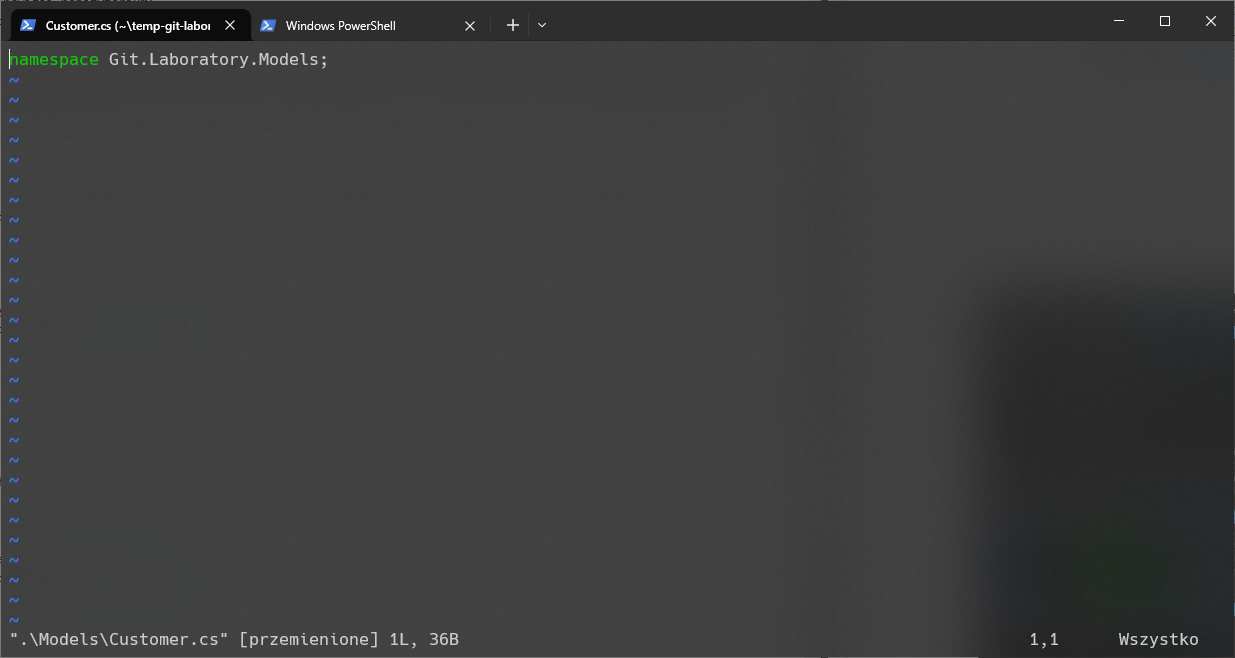
\includegraphics [scale=0.5]{customer-beforeDiff.PNG}}
    \label{fig:label}
\end{figure}
\vspace*{\fill}
\newpage

\vspace*{\fill}
\begin{figure}[!h]
    \caption{Zawartość pliku Customer.cs po zmianie}
    \centerline{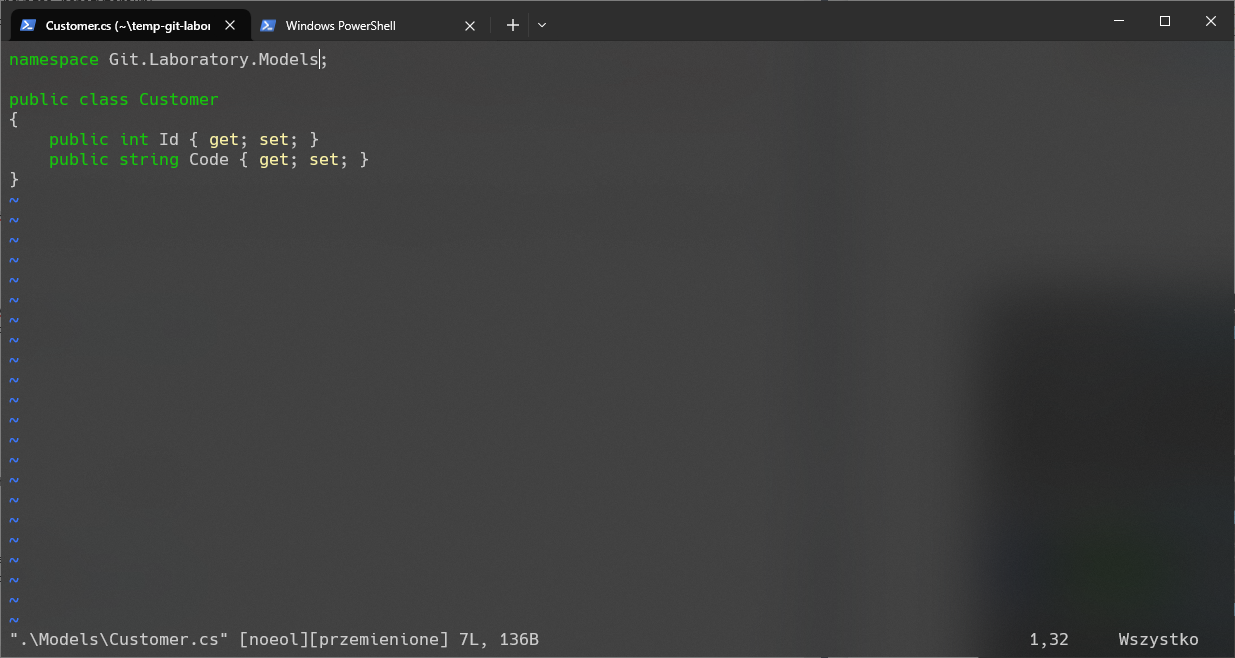
\includegraphics [scale=0.5]{customer-afterDiff.PNG}}
    \label{fig:label}
\end{figure}
\vspace*{\fill}
\newpage

\vspace*{\fill}
\begin{figure}[!h]
    \caption{Rezultatu wykonania git-diff}
    \centerline{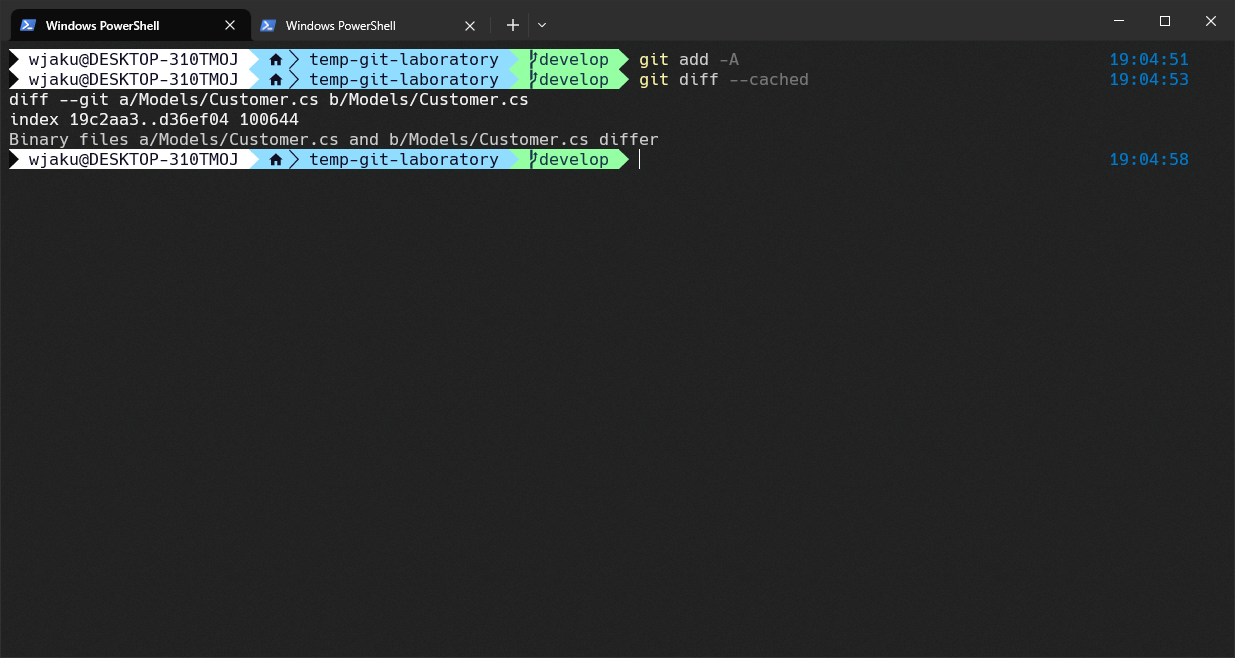
\includegraphics [scale=0.5]{git-diff.PNG}}
    \label{fig:label}
\end{figure}
\vspace*{\fill}
\newpage

\section{Łącznie gałęzi - git merge}

Łączenie zawartości gałęzi develop z gałęzią master. W celu lepszego pokazania struktury rewizji oraz istoty samego merge'a, przed łączniem utworzyłem commita na gałęzi master.

\vspace*{\fill}
\begin{figure}[!h]
    \caption{Wykonanie git merge}
    \centerline{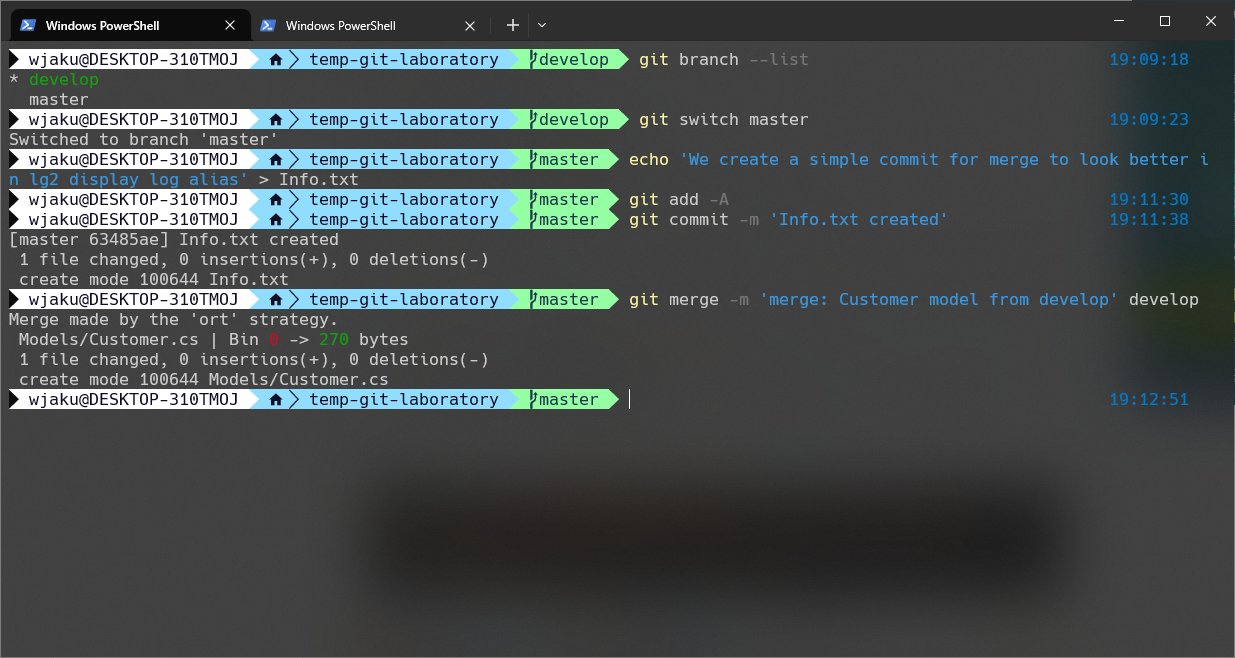
\includegraphics [scale=0.5]{merge.PNG}}
    \label{fig:label}
\end{figure}
\vspace*{\fill}
\newpage

\vspace*{\fill}
\begin{figure}[!h]
    \caption{Rezultat git merge}
    \centerline{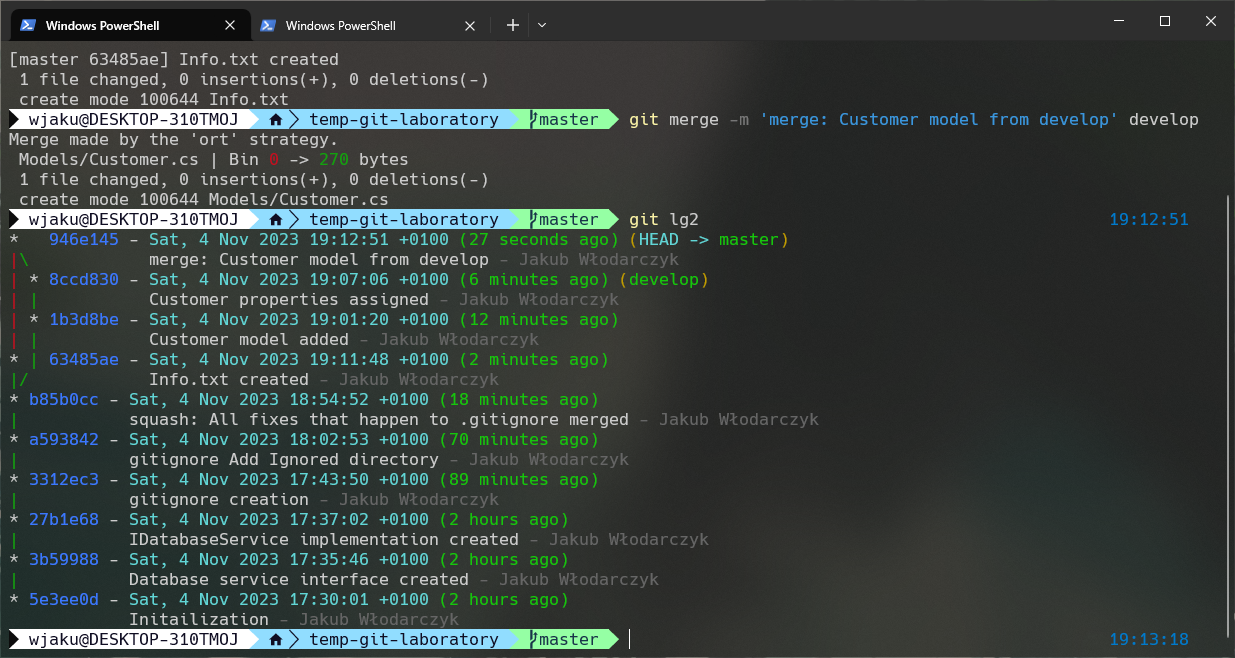
\includegraphics [scale=0.5]{merge-result.PNG}}
    \label{fig:label}
\end{figure}
Przedstawiony log również jest aliasem, jego dokładny kod zawiera się w obrebie Rysunku 17.
\vspace*{\fill}
\newpage

\end{document}
